\documentclass[tikz,border=4pt]{standalone}
\usepackage{amsmath,amssymb}

\usetikzlibrary{arrows.meta,positioning,automata,shapes,shapes.misc,calc,decorations.pathmorphing,decorations.markings,angles,quotes,patterns,mindmap,matrix,knots,hobby,trees}
\tikzset{->-/.style={decoration={markings, mark=at position 0.5 with {\arrow{Stealth}}}, postaction={decorate}}}
\begin{document}
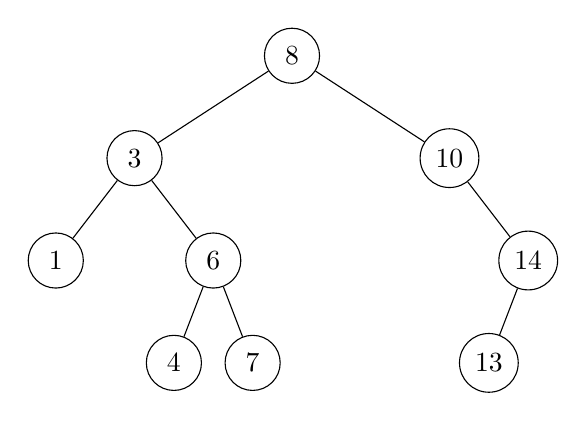
\begin{tikzpicture}[level distance=1.3cm, level 1/.style={sibling distance=4cm}, level 2/.style={sibling distance=2cm}, level 3/.style={sibling distance=1cm}, every node/.style={circle, draw, minimum size=7mm}]
\node {8}
  child { node {3} child { node {1} } child { node {6} child { node {4} } child { node {7} } } }
  child { node {10} child[missing] child { node {14} child { node {13} } child[missing] } };
\end{tikzpicture}
\end{document}
